% =============================================================================
% COPYRIGHT AND DISCLAIMER
% =============================================================================
% This file is provided as a convenience template for competition participants.
% By using it, you accept full responsibility for compliance with all applicable
% copyright, licensing, and usage rules of the Association for Computing
% Machinery (ACM) and of any LaTeX packages you load (including, without
% limitation, the "acmart" document class and related ACM materials).
%
% Consult ACM's official publication, template, and copyright policies before
% using this setup for any purpose other than this competition. Do not assume
% that this template may be reused, redistributed, or submitted elsewhere
% without independently verifying ACM's current rules.
%
% Use of the "acmart" class, the "sigconf" option, or ACM-style formatting in
% this template does NOT mean that this report, this competition, its organizers,
% or any resulting PDF is sponsored, endorsed, affiliated with, or published by
% ACM. ACM trademarks and branding remain the property of ACM.
%
% Template packages live in preamble.tex.
% Citations live in main.bib. Edit this file with your paper content.
% =============================================================================

\documentclass[sigconf]{acmart}
% =============================================================================
% Template setup — participants normally do not edit this file.
% Author content belongs in main.tex; citations belong in main.bib.
% \documentclass lives in main.tex so Overleaf does not treat this file as root.
% =============================================================================

% --- Competition / non-ACM-submission friendly rights metadata -------------
\setcopyright{none}
\settopmatter{printacmref=false}
\acmConference[Kaggle Competition]{Filament Segmentation Challenge}{2026}{\href{https://www.kaggle.com/competitions/filament-segmentation-2026}{kaggle.com/competitions/filament-segmentation-2026}}
\acmBooktitle{Competition Report}
\acmDOI{}
\acmISBN{}

% --- Author guidance text --------------------------------------------------
% \guide{...} is gray italic while \guideStyletrue; omitted from the PDF if false.
% Flip the switch in main.tex after % =============================================================================
% Template setup — participants normally do not edit this file.
% Author content belongs in main.tex; citations belong in main.bib.
% \documentclass lives in main.tex so Overleaf does not treat this file as root.
% =============================================================================

% --- Competition / non-ACM-submission friendly rights metadata -------------
\setcopyright{none}
\settopmatter{printacmref=false}
\acmConference[Kaggle Competition]{Filament Segmentation Challenge}{2026}{\href{https://www.kaggle.com/competitions/filament-segmentation-2026}{kaggle.com/competitions/filament-segmentation-2026}}
\acmBooktitle{Competition Report}
\acmDOI{}
\acmISBN{}

% --- Author guidance text --------------------------------------------------
% \guide{...} is gray italic while \guideStyletrue; omitted from the PDF if false.
% Flip the switch in main.tex after % =============================================================================
% Template setup — participants normally do not edit this file.
% Author content belongs in main.tex; citations belong in main.bib.
% \documentclass lives in main.tex so Overleaf does not treat this file as root.
% =============================================================================

% --- Competition / non-ACM-submission friendly rights metadata -------------
\setcopyright{none}
\settopmatter{printacmref=false}
\acmConference[Kaggle Competition]{Filament Segmentation Challenge}{2026}{\href{https://www.kaggle.com/competitions/filament-segmentation-2026}{kaggle.com/competitions/filament-segmentation-2026}}
\acmBooktitle{Competition Report}
\acmDOI{}
\acmISBN{}

% --- Author guidance text --------------------------------------------------
% \guide{...} is gray italic while \guideStyletrue; omitted from the PDF if false.
% Flip the switch in main.tex after \input{preamble}.
%
% Do not use \guide{...} for \email{...}.
\usepackage{xcolor}
\newif\ifguideStyle
\guideStyletrue
\newcommand{\guide}[1]{%
  \ifguideStyle
    {\color{gray!65}\itshape #1}%
  \fi
}

% --- Math ------------------------------------------------------------------
% Do NOT load amssymb (or amsfonts): acmart already loads newtxmath, which
% defines the same symbols (e.g. \Bbbk) and causes a conflict on Overleaf.
% amsmath is already provided by acmart; mathtools extends it.
\usepackage{mathtools}

% --- Figures ---------------------------------------------------------------
% graphicx is already loaded by acmart
\usepackage{subcaption}

% --- Tables ----------------------------------------------------------------
% booktabs is already loaded by acmart
\usepackage{tabularx}
\usepackage{multirow}

% --- Bibliography style is set in main.tex (ACM-Reference-Format) ----------
.
%
% Do not use \guide{...} for \email{...}.
\usepackage{xcolor}
\newif\ifguideStyle
\guideStyletrue
\newcommand{\guide}[1]{%
  \ifguideStyle
    {\color{gray!65}\itshape #1}%
  \fi
}

% --- Math ------------------------------------------------------------------
% Do NOT load amssymb (or amsfonts): acmart already loads newtxmath, which
% defines the same symbols (e.g. \Bbbk) and causes a conflict on Overleaf.
% amsmath is already provided by acmart; mathtools extends it.
\usepackage{mathtools}

% --- Figures ---------------------------------------------------------------
% graphicx is already loaded by acmart
\usepackage{subcaption}

% --- Tables ----------------------------------------------------------------
% booktabs is already loaded by acmart
\usepackage{tabularx}
\usepackage{multirow}

% --- Bibliography style is set in main.tex (ACM-Reference-Format) ----------
.
%
% Do not use \guide{...} for \email{...}.
\usepackage{xcolor}
\newif\ifguideStyle
\guideStyletrue
\newcommand{\guide}[1]{%
  \ifguideStyle
    {\color{gray!65}\itshape #1}%
  \fi
}

% --- Math ------------------------------------------------------------------
% Do NOT load amssymb (or amsfonts): acmart already loads newtxmath, which
% defines the same symbols (e.g. \Bbbk) and causes a conflict on Overleaf.
% amsmath is already provided by acmart; mathtools extends it.
\usepackage{mathtools}

% --- Figures ---------------------------------------------------------------
% graphicx is already loaded by acmart
\usepackage{subcaption}

% --- Tables ----------------------------------------------------------------
% booktabs is already loaded by acmart
\usepackage{tabularx}
\usepackage{multirow}

% --- Bibliography style is set in main.tex (ACM-Reference-Format) ----------


% Guide styling: \guideStyletrue = show gray italic hints; \guideStylefalse = omit them
\guideStylefalse

\begin{document}
\emergencystretch=1.5em % lets a line stretch instead of running into the margin

\title{A Two-Lane Candidate Pool with a Metric-Derived Selector}
\subtitle{A Solution to the Solar Filament Segmentation Challenge 2026} % DO NOT CHANGE

\author{Talha Bacak}
\affiliation{%
  \city{Ankara}
  \country{Türkiye}
}
\email{talhadhh@gmail.com}

\begin{abstract}
    This report describes our solution to the Solar Filament Segmentation Challenge~2026, a Kaggle competition on automatic segmentation of solar filaments in GONG H-$\alpha$ observations. Two independent lanes propose filament instances on the full-disc frame: a YOLO11m-seg detector and a twelve-member U-Net ensemble. The candidates are fused by confidence-weighted voting, described by 42 features, and kept or dropped by a bagged gradient-boosted selector whose keep threshold is derived from the Panoptic Quality formula instead of being tuned. Out of fold on all 707 training images the system reaches PQ 0.443 (95\,\% interval 0.434--0.452), where one annotator scored against the others reaches 0.340; the public leaderboard displays 0.40. The repository rebuilds the submitted file byte for byte.
\end{abstract}

\maketitle

% ==================================== %
%              INTRODUCTION            %
% ==================================== %
\section{Introduction}
    This report goes over the details of our submitted solution to the Solar Filament Segmentation Challenge~2026 \cite{filament-segmentation-2026}. The challenge, launched on July~10,~2026, is organized by the Earth-Space AI Research (ESAIR) Lab\footnote{\href{https://www.esairlab.com/home}{www.esairlab.com/}}. This challenge utilizes the MAGFiLO dataset for evaluation of the segmentation algorithms \cite{ahmadzadeh2024dataset}. Our solution combines existing components (a YOLO11 instance detector, U-Net semantic models and gradient-boosted trees). Every parameter below was adopted on a pooled five-fold out-of-fold measurement with the competition's own scorer, and the changes that were measured and rejected are reported in Section~\ref{sec:evaluation}. Code, weights and the record of all experiments are public\footnote{\url{https://github.com/talhabacak/solar-filament-segmentation-2026}}. The public MAGFiLO release contains annotations for all 180 test images; we verified this at the identifier level in the first week, quarantined the release, and never used it for training, model selection or prediction.

% ==================================== %
%              METHODOLOGY             %
% ==================================== %
\section{Methodology}\label{sec:methodology}

\subsection{Metric and its consequences}
The competition scores Panoptic Quality \cite{kirillov2019panoptic},
\begin{equation}
  \mathrm{PQ}=\frac{\sum_{(g,p)\in \mathit{TP}}\mathrm{IoU}(g,p)}{|\mathit{TP}|+\tfrac12|\mathit{FP}|+\tfrac12|\mathit{FN}|},
  \label{eq:pq}
\end{equation}
with a match requiring $\mathrm{IoU}>0.5$, pooled over annotator-image entries: an image annotated by several people is scored once against each annotator's copy. Three consequences shaped the design. The task is instance reconstruction, since a correct probability map that merges two filaments loses two matches. The reward is discontinuous at IoU 0.5, so the last stage must decide which candidates to keep. And Eq.~\ref{eq:pq} prices that decision, which Section~\ref{sec:selector} uses. Figure~\ref{fig:pipeline} shows the resulting pipeline and Table~\ref{tab:params} lists every parameter.

\begin{figure*}[t]
  \centering
  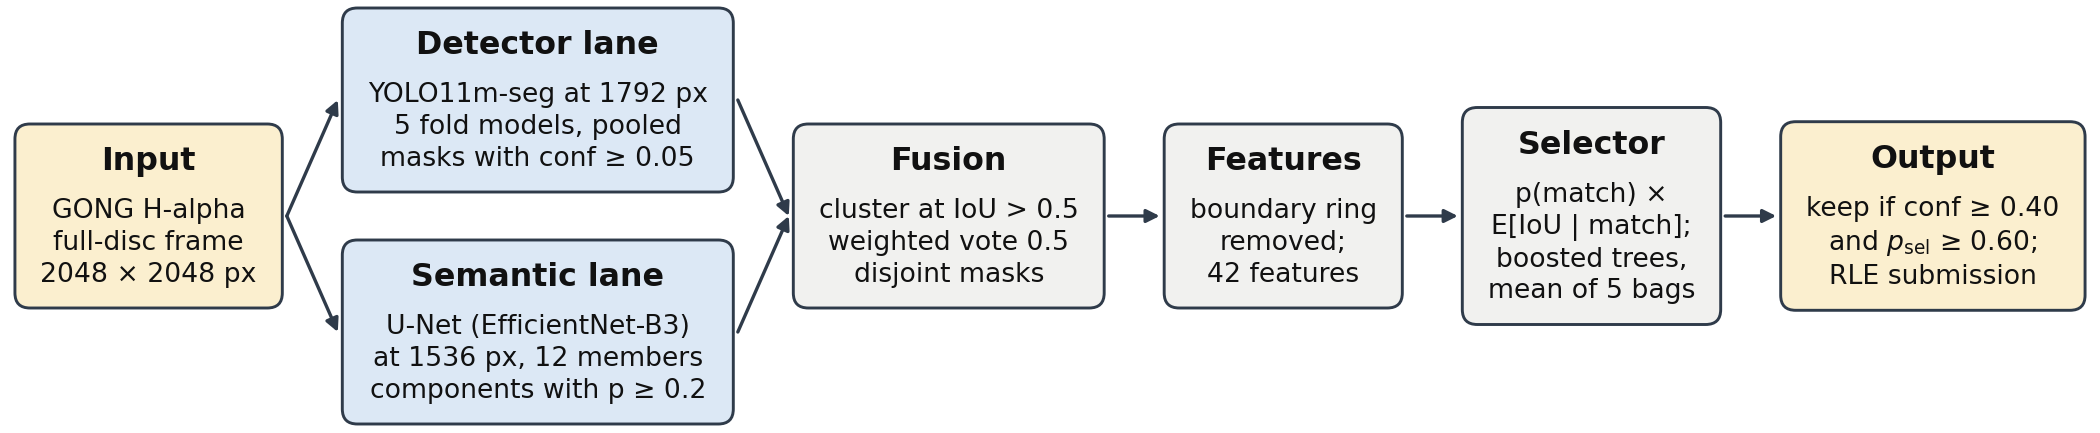
\includegraphics[width=\textwidth]{figures/pipeline.png}
  \caption{The pipeline. Two lanes propose instance candidates independently; fusion turns them into one pixel-disjoint candidate pool; a learned selector decides which candidates are written to the submission.}
  \Description{A flow diagram from the input image through a detector lane and a semantic lane to fusion, features, selector and output.}
  \label{fig:pipeline}
\end{figure*}

\subsection{Data, splits and validation protocol}\label{sec:protocol}
The data are 707 training and 180 test frames ($2048\times2048$, 8-bit JPEG) from the six GONG stations, with 8199 polygon annotations in 1154 annotator-image entries. The solar disc is centred at $(1023.6, 1024.6)$\,px with radius 899.95\,px (standard deviation 0.73\,px over all 887 frames), so no geometric registration is applied.

There is no separate held-out set: the training images are split into five folds with \texttt{GroupKFold} grouped by physical image, so that all annotator entries of an image share a fold. The assignment was frozen once (\texttt{data/splits/folds\_v1.parquet}) and used unchanged by every experiment. Every learned layer is cross-fitted. Network predictions for a training image come only from the fold model that did not see it, and the selector is fitted on four folds and applied to the fifth. The semantic lane is trained on every annotator entry, because the metric scores against every copy. The five detectors are trained on one copy per image, the medoid annotator's; an all-copies detector later measured $+0.0051$ PQ on fold 0, but the production detectors were not retrained. At test time the five fold models act as an ensemble.

\subsection{Pre-processing}
Images are used as delivered. There is no contrast equalisation, intensity harmonisation or limb-darkening correction. For the semantic lane the frame is resized once to $1536\times1536$, scaled to $[0,1]$ and replicated to three channels. Masks are downsampled by area averaging and thresholded at 0.5, which retains 98.1\,\% of the annotated area and deletes no instance. The detector uses the Ultralytics input pipeline at 1792\,px.

\subsection{Detector lane}
YOLO11m-seg \cite{yolo11}, initialised from COCO weights \cite{lin2014coco}, single class, one model per fold. Augmentations that break the full-disc geometry (mosaic, mixup, copy-paste, erasing, shear, perspective, vertical flip) are off. Candidates are kept at confidence $\geq 0.05$. NMS is at IoU 0.5 for the out-of-fold candidates the selector is trained on but at 0.05 for the test-time candidates, a difference we found when reproducing the system. Measured afterwards on fold 0 with that fold's out-of-fold selector, the test setting removes 188 of 1927 candidates, none of them a match, and changes PQ by $+0.0007$ [$-0.0043$, $+0.0055$]. In a sweep of input sizes from 1024 to 2048\,px, 1792 is the last that improves; larger backbones did not help.

\subsection{Semantic lane}
U-Net \cite{ronneberger2015unet} with an ImageNet-initialised \cite{deng2009imagenet} EfficientNet-B3 encoder \cite{tan2019efficientnet} and scSE decoder attention \cite{roy2018scse}, built with Segmentation Models PyTorch \cite{smp}. The loss is BCE + soft Dice + $0.3\cdot$clDice \cite{shit2021cldice}; clDice rewards skeleton overlap, because a one-pixel break splits an instance and PQ charges it twice. Three member types are trained: (a) the base recipe, one model per fold; (b) an instance-balanced variant, one per fold, trained for 60 epochs with the heavy augmentation of (c), whose loss weights each connected instance equally within a 40\,px radius, so that small filaments count as much as large ones; (c) two heavily augmented models trained for 60 epochs at 768 and 1536\,px on the fold-0 split. The test-time field is their weighted mean, 0.50 for (b), 1/6 for (a) and 1/6 for each model of (c), each member inferred at its training size with horizontal-flip averaging.

\begin{table}[t]
  \caption{All parameters of the submitted system.}
  \label{tab:params}
  \small
  \begin{tabular}{@{}p{0.22\columnwidth}p{0.74\columnwidth}@{}}
    \toprule
    Component & Setting \\
    \midrule
    Detector & YOLO11m-seg, 1792\,px, single class, medoid targets, 40 epochs, patience 15, batch 2, optimizer \texttt{auto} (resolves to AdamW, lr 0.002, momentum 0.9), lrf 0.01, weight decay 5e-4, warm-up 3 epochs \\
    Detector augmentation & rotation $\pm10^\circ$, translate 0.05, scale 0.10, horizontal flip 0.5, brightness 0.3; all others off \\
    Semantic model & U-Net, EfficientNet-B3, scSE, 1536\,px, batch 2, AdamW lr 3e-4, weight decay 1e-4, OneCycle (pct\_start 0.1), mixed precision, 30 epochs (instance-balanced and heavy members 60) \\
    Semantic loss & BCE + Dice + $0.3\cdot$clDice (5-epoch warm-up); instance-balanced variant: radius 40\,px, weight 1.0 \\
    Semantic augmentation & horizontal flip 0.5, rotation $\pm10^\circ$ about the disc centre, gamma 0.8--1.25; instance-balanced and heavy members: flips, $90^\circ$ rotations, $\pm20^\circ$, station-calibrated photometry \\
    Fusion & semantic threshold 0.2, minimum area 256\,px, cluster IoU 0.5, vote 0.5, detector NMS 0.5 out of fold and 0.05 at test time, at most 300 detections \\
    Selector & classifier: 300 iterations, lr 0.05, 31 leaves, minimum leaf 25, L2 1.0; regressor: 300 iterations, lr 0.06; 5 image-bootstrap copies; 10\,042 training candidates \\
    Keep rule & confidence $\geq 0.40$ and $p_\mathrm{sel}\geq 0.60$ \\
    \bottomrule
  \end{tabular}
\end{table}

\subsection{Fusion and features}
Per image, detector masks (confidence $\geq 0.05$, centroid $r/R\leq 0.97$) and connected components of the semantic field ($p\geq 0.2$, area $\geq 256$\,px) are clustered by union-find at $\mathrm{IoU}>0.5$. Each cluster becomes one mask by confidence-weighted pixel voting at 0.5, and masks are made pixel-disjoint greedily in confidence order, as the submission format requires. Each candidate receives 42 features from one shared function used at training and at test time: geometry (area, elongation, skeleton length, width), position on the disc, semantic support (probability statistics, ring contrast), detector support (per-model confidence, agreement, vote count), candidate density, photometry of the raw frame and structure-tensor orientation.

\subsection{Selector and keep rule}\label{sec:selector}
The selector is two histogram gradient-boosting models \cite{pedregosa2011sklearn}: a classifier for ``this candidate matches some annotator copy'' multiplied by a regressor, fitted on positives only, for the IoU summed over the copies it matches. The product is mapped to a quantile of its out-of-fold distribution, giving a score $p_\mathrm{sel}$. The submitted selector averages five such pairs, each fitted on a bootstrap sample of images. The keep rule follows from Eq.~\ref{eq:pq}: adding a candidate raises PQ when its expected copy-weighted IoU sum exceeds $\tfrac12\,c\,\mathrm{PQ}$, where $c$ is the mean number of copies per image; this is 0.361 at our operating point. Measured calibration crosses that value between the score bands 0.55--0.60 (0.364) and 0.60--0.65 (0.485), so the gate is confidence $\geq 0.40$ and $p_\mathrm{sel}\geq 0.60$.

\subsection{Post-processing and submission}
Before featurisation each mask loses its one-pixel boundary ring, which corrects a measured tendency of our contours to enclose the annotators' ($+0.0128$ PQ). Masks under 64\,px are dropped and the rest are written as run-length encodings. The final submission holds 1117 instances on 177 of 180 images (Figure~\ref{fig:examples}).

\begin{figure*}[t]
  \centering
  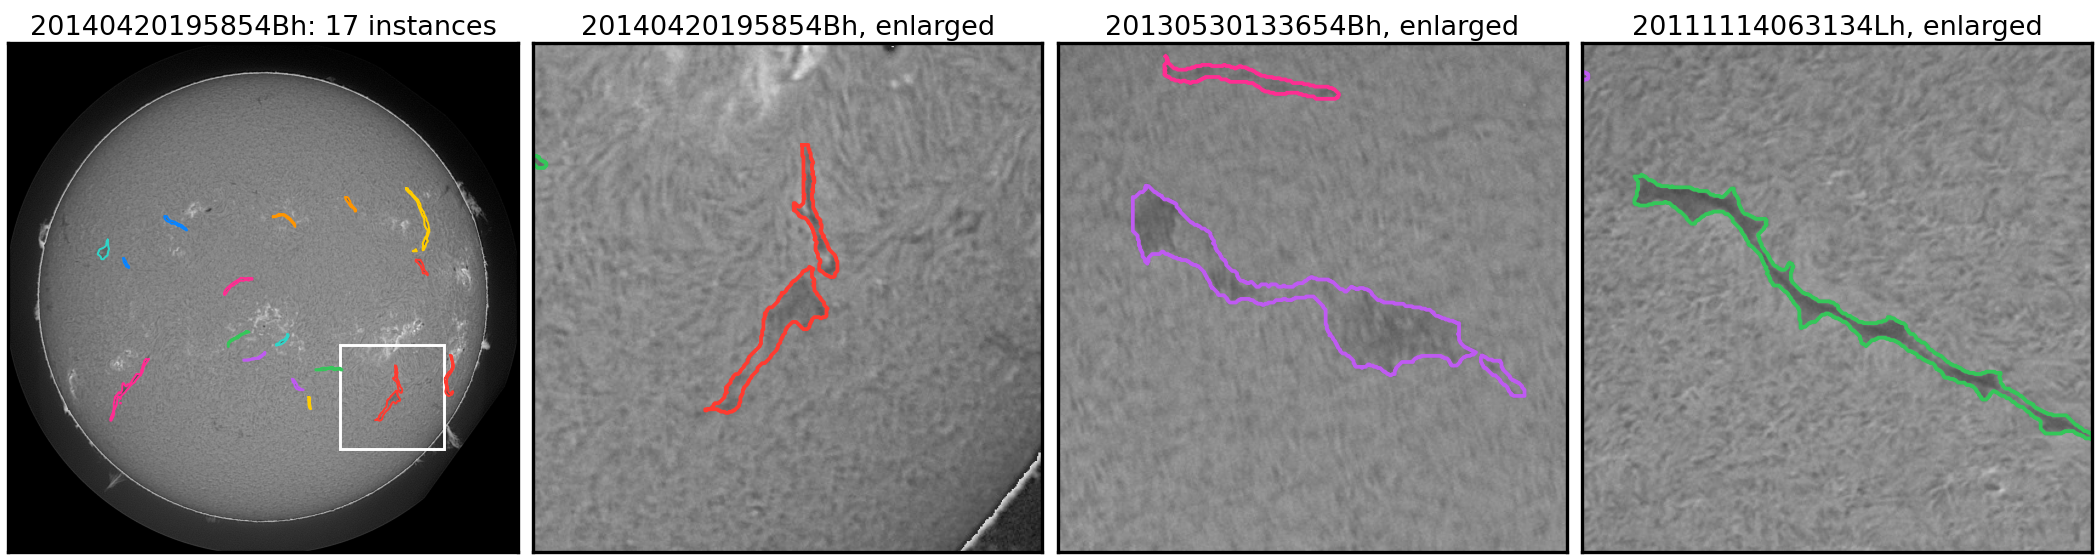
\includegraphics[width=0.78\textwidth]{figures/examples.png}
  \caption{The final submission on test images: a full-disc frame with every predicted instance outlined, and enlarged regions of that frame and of two frames from other years. The frames are chosen by rule (most predicted instances).}
  \Description{A full-disc H-alpha image with coloured outlines of predicted filaments, and three enlarged regions showing outlines that follow dark elongated filaments.}
  \label{fig:examples}
\end{figure*}

% ==================================== %
%              EVALUATION              %
% ==================================== %
\section{Evaluation}\label{sec:evaluation}

\subsection{Strategy}
All scores are pooled over the five held-out folds (Section~\ref{sec:protocol}) with our implementation of Eq.~\ref{eq:pq}, which is tested for equality with the organisers' published scorer. Intervals are 95\,\% bootstrap intervals over images (4000 resamples). A change is adopted only if a paired bootstrap places it above a pre-registered floor of $\pm0.003$: a seed replicate of one ensemble member moves PQ by $\pm0.001$, and the same selector variant re-read on five different fold partitions moves with standard deviation 0.0015.

\subsection{Results}
Table~\ref{tab:results} scores simpler systems built from the same components, between two human references: one annotator scored against the others, and a majority-consensus mask built from every annotator's drawing. The thresholds of the three reference systems were chosen in sample, which favours them. The semantic lane alone beats the detector alone, fusing them adds $+0.021$, and the learned selector adds $+0.009$ more, all of it precision: it removes 840 false positives at a cost of 289 true positives. For the full system the intervals are PQ $[0.434, 0.452]$, SQ $[0.675, 0.681]$ and RQ $[0.641, 0.665]$; the five folds read 0.451, 0.447, 0.448, 0.458 and 0.412.

\begin{table}[t]
  \caption{Out-of-fold results on the 707 training images.}
  \label{tab:results}
  \small\setlength{\tabcolsep}{4.2pt}
  \begin{tabular}{@{}lrrrrrr@{}}
    \toprule
    System & PQ & SQ & RQ & TP & FP & FN \\
    \midrule
    One annotator vs.\ the others & 0.340 & 0.634 & 0.536 & & & \\
    Detector only & 0.398 & 0.665 & 0.598 & 4492 & 2339 & 3707 \\
    Semantic lane only & 0.413 & 0.677 & 0.610 & 5273 & 3810 & 2926 \\
    Fusion, confidence gate & 0.434 & 0.675 & 0.643 & 5106 & 2569 & 3093 \\
    \textbf{Full system} & \textbf{0.443} & 0.678 & 0.653 & 4817 & 1729 & 3382 \\
    Consensus of all annotators & 0.641 & 0.790 & 0.812 & & & \\
    \bottomrule
  \end{tabular}
\end{table}

Over the matched copies, IoU has median 0.683 (quartiles 0.615 and 0.742; 5th and 95th percentiles 0.533 and 0.810) and Dice has median 0.812 (quartiles 0.762 and 0.852; 5th and 95th percentiles 0.695 and 0.895). Table~\ref{tab:relations} gives the relation distributions with the definition of the organisers' self-evaluation notebook: fragmentation and merging are each near 2--3\,\%, and the rest of the unmatched mass is pure misses and pure extras. These distributions are read before selector bagging (PQ 0.4421); bagging adds $+0.0010$.

\begin{table}[t]
  \caption{One-to-many (fragmentation) and many-to-one (merging) relations, out of fold.}
  \label{tab:relations}
  \small
  \begin{tabular}{@{}lrrr@{}}
    \toprule
    Side & one & two or more & none \\
    \midrule
    Ground truth $\rightarrow$ predictions & 69.9\,\% & 2.1\,\% & 28.0\,\% \\
    Predictions $\rightarrow$ ground truth & 87.8\,\% & 2.6\,\% & 9.6\,\% \\
    \bottomrule
  \end{tabular}
\end{table}

The public leaderboard displays 0.40. The offset of $-0.04$ to $-0.05$ from the local estimate has been the same for every generation of the pipeline. Scoring the same masks against different annotators moves PQ by $-0.036$ to $+0.038$, so we attribute the offset to the test annotators and expect 0.40 to 0.42 on the private half. For the 180 test images, each of the twelve semantic members takes about 21\,s on one GPU, and fusion with featurisation takes 0.48\,s per image on a CPU.

\subsection{Strengths}
Mask quality is at the reproducibility of the label: on the 2483 matched copies that two annotators drew, our mask is closer to an annotator than the second annotator is in 76.2\,\% of cases (SQ 0.678 against an inter-annotator IoU of 0.634). The instance structure is clean (Table~\ref{tab:relations}). The sixteen scored false positives with the highest selector score are all visibly filaments that no annotator of that image drew, so part of the false-positive count is recall of real structure.

\subsection{Weaknesses and strategies for improvement}
The remaining loss is recognition: recall is 0.588 at precision 0.736. Of the on-disc annotator copies, 60.6\,\% are matched, 11.5\,\% had a candidate above IoU 0.5 that the selector rejected, 3.4\,\% were never proposed, and 24.6\,\% have a candidate with IoU between 0.05 and 0.5, the right object with the wrong shape. Where a second annotator confirms such a copy, our candidate is too short, not too thin (median skeleton ratio 0.72, width ratio 1.04), and in 75\,\% of these cases the ensemble's probability is essentially zero over the missing part. Barbs show the same limit (Figure~\ref{fig:barbs}). Defining a barb pixel from the annotated spine as one thinner than the body and farther from the spine than half a body width, our matched masks cover 38.0\,\% of barb pixels where a second annotator covers 49.3\,\%, against 80.5\,\% and 79.7\,\% of the body. Recognition also falls at the limb (RQ 0.556 for $r/R$ in 0.8--0.9, against 0.66--0.67 on the disc), while SQ stays at 0.68.

\begin{figure}[t]
  \centering
  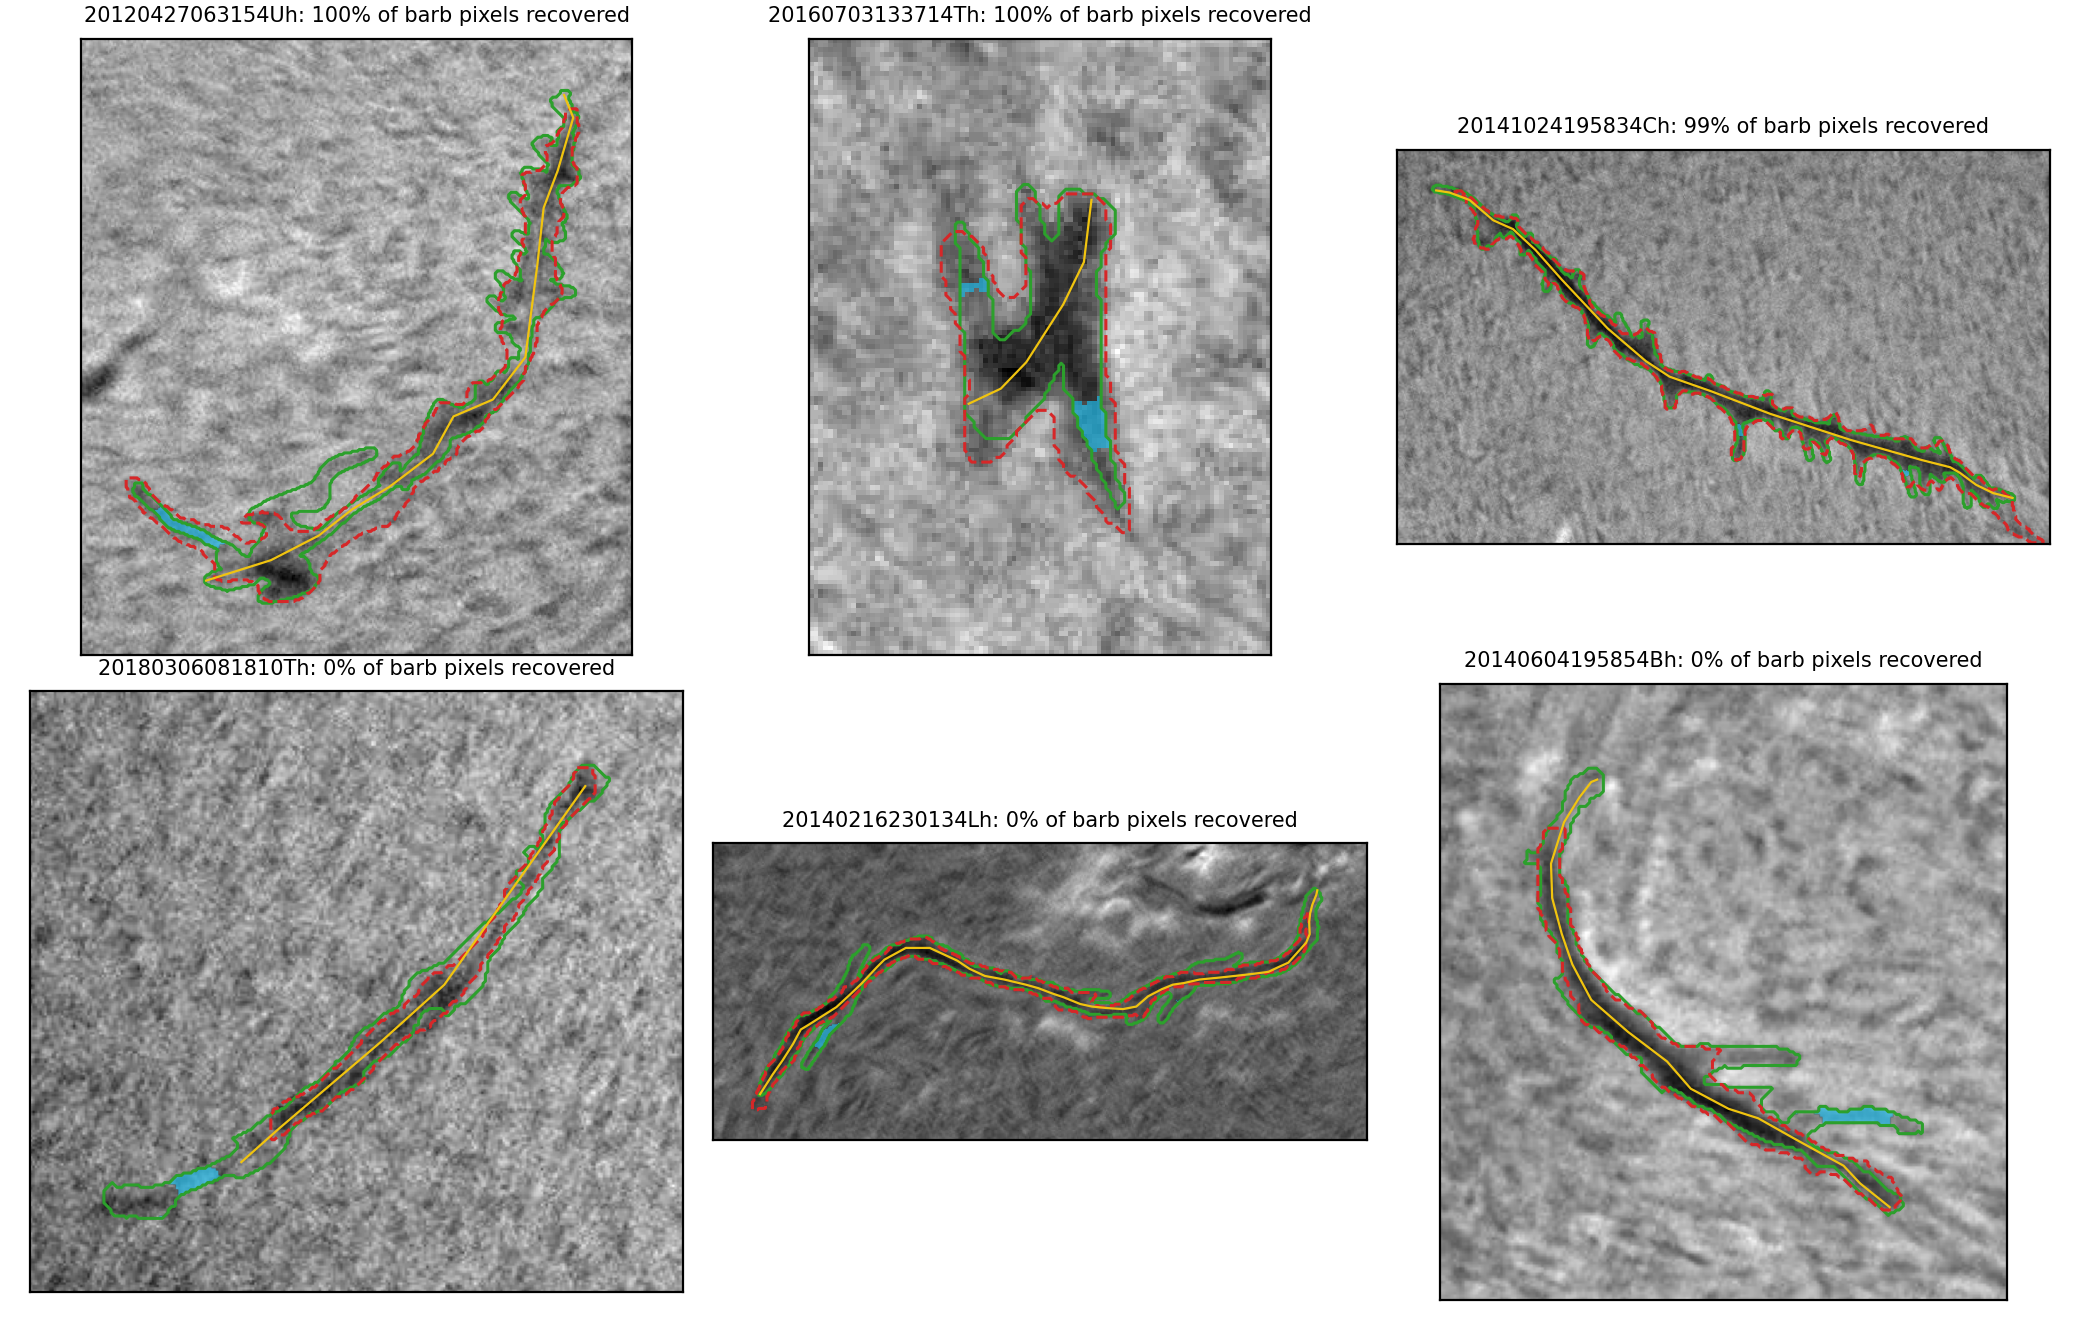
\includegraphics[width=0.70\columnwidth]{figures/barbs.png}
  \caption{Barbs (shaded) of annotated training filaments with the annotator's outline (solid), our out-of-fold mask (dashed) and the annotated spine. Top row: the three matched copies whose barbs are recovered best; bottom row: the three recovered least.}
  \Description{Six enlarged H-alpha regions with annotator outlines, predicted outlines and spines; short barbs attached to dark bodies are followed and long faint ones are not.}
  \label{fig:barbs}
\end{figure}

Table~\ref{tab:negative} lists changes that were implemented and measured under the same protocol and did not pass the floor. They locate the limit in the networks' response to faint structure, not in fusion, selection or post-processing: moving the fusion vote towards the union costs $-0.058$ PQ, snapping masks to image intensity costs $-0.070$, and the apparent headroom of selection (reordering the pool with knowledge of one annotator, $+0.033$) is lost when the same choice is scored on another annotator. We therefore see two directions. First, supervision aimed at faint length and barbs, for which PQ itself gives no incentive (barbs are 0.17\,\% of the annotated area). Second, labels with several annotators per image: 66.5\,\% of the wrong-shape copies were drawn by one annotator only, and the consensus oracle shows how much of the gap is label variance.

\begin{table}[t]
  \caption{Measured changes that did not pass the $\pm0.003$ floor.}
  \label{tab:negative}
  \small
  \begin{tabular}{@{}p{0.55\columnwidth}p{0.41\columnwidth}@{}}
    \toprule
    Change & Measured effect \\
    \midrule
    Nine encoders (13--93\,M parameters), UNet++, UPerNet, SegFormer as a member & within $\pm0.001$ of a seed replicate \\
    Mask2Former as a third lane & $+0.0020$ $[-0.0027, +0.0066]$ \\
    Candidate-conditioned mask refiner & best of three $-0.015$ \\
    Pretraining on unlabelled GONG frames & equal to a seed replicate \\
    HMI magnetogram as teacher input & $+0.0015$, $+0.0003$ (two folds) \\
    Semantic threshold 0.10, selector refitted & $+0.0010$ $[-0.0019, +0.0038]$ \\
    Keep threshold set by image regime & $+0.0019$ $[-0.0006, +0.0044]$ \\
    Cascade over the band $0.40\leq p_\mathrm{sel}<0.60$ & $+0.0008$ $[-0.0011, +0.0026]$ \\
    \bottomrule
  \end{tabular}
\end{table}

% ==================================== %
%      REPRODUCIBILITY AND COMPLIANCE  %
% ==================================== %
\section{Reproducibility and compliance}\label{sec:repro}
The repository is modular (metric, cache builders, training and inference, one script per measurement) and \texttt{requirements.txt} pins every package. The notebook in \texttt{notebooks/} runs the pipeline in three modes: the final stage from the shipped test candidate pool (CPU, seconds), full inference from the released weights, or a complete retrain. From the candidate pool the submitted file is rebuilt byte for byte, also after refitting the selector from the shipped training pool.

No external annotation was used. ImageNet encoder weights and COCO-pretrained detector weights are the only external inputs to the submitted models; magnetograms and unlabelled GONG frames appear only in experiments of Table~\ref{tab:negative}, and inference reads only the provided H-$\alpha$ images. AI tools were used for coding and drafting, as the organisers permit; every design decision above traces to a recorded measurement in the repository.

% ==================================== %
%            ACKNOWLEDGMENT            %
% ==================================== %
\section{Acknowledgment}\label{sec:acknowledgment}
    % Do not change
    The organization of the Filament Segmentation Challenge 2026 is partially supported by the U.S. National Science Foundation (NSF) under Grant No. 2209912 and 2433781, directorate for Computer and Information Science and Engineering (CSE), and Office of Advanced Cyberinfrastructure (OAC), and Grant No. 2511630, AST Division Of Astronomical Sciences and MPS Directorate for Mathematical and Physical Sciences.

    The Filament Segmentation Challenge 2026 is sponsored by the U.S. National Science Foundation (NSF) National Solar Observatory (NSO).

    This work utilizes GONG data obtained by the NSO Integrated Synoptic Program, managed by the National Solar Observatory, which is operated by the Association of Universities for Research in Astronomy (AURA), Inc. under a cooperative agreement with the National Science Foundation and with contribution from the National Oceanic and Atmospheric Administration. The GONG network of instruments is hosted by the Big Bear Solar Observatory, High Altitude Observatory, Learmonth Solar Observatory, Udaipur Solar Observatory, Instituto de Astrofísica de Canarias, and Cerro Tololo Interamerican Observatory.

\bibliographystyle{ACM-Reference-Format}
\bibliography{main}

\end{document}
